% answers.tex —— 2006 年·普通高等学校招生考试·福建卷文科 · 参考答案与详细解析片段
% 由 tools/generate_projects.py 依来源总账自 2006/2006_数学真题_福建文_试题.md + 2006/2006_数学真题_福建文_解析正文.md + 2006/2006_数学真题_福建文_答案要点.md 生成，勿手改（改源 MD 后重跑）


\begin{gktip}
以下各题为依据规范题面自行推导并复算的非官方解析；固定候选 PDF 未见答案、解析或评分标准。来源身份未核。Q19、Q20 的解答仅使用题面明确给出的文字条件，不以待重绘图形补充条件。
\end{gktip}

\begin{answer}
\gksolhead{1}{}

\textbf{题目}：

已知两条直线 $y=ax-2$ 和 $y=(a+2)x+1$ 互相垂直，则 $a$ 等于\mbox{（　　）}

（A）$2$　　（B）$1$　　（C）$0$　　（D）$-1$

\Needspace{4\baselineskip}
\textbf{解析}

两条直线斜率为 $a$ 与 $a+2$。垂直条件给出 $a(a+2)=-1$，即 $(a+1)^2=0$，所以 $a=-1$，选 D。代入后斜率为 $-1$ 与 $1$，乘积为 $-1$。

\gkanswer{答案：D，$a=-1$}

\end{answer}
\begin{answer}
\gksolhead{2}{}

\textbf{题目}：

在等差数列 $\{a_n\}$ 中，已知 $a_1=2$，$a_2+a_3=13$，则 $a_4+a_5+a_6$ 等于\mbox{（　　）}

（A）$40$　　（B）$42$　　（C）$43$　　（D）$45$

\Needspace{4\baselineskip}
\textbf{解析}

设公差为 $d$，则 $a_2=2+d$、$a_3=2+2d$。由 $a_2+a_3=13$ 得 $4+3d=13$，故 $d=3$。于是 $a_4+a_5+a_6=11+14+17=42$，选 B。

\gkanswer{答案：B，$42$}

\end{answer}
\begin{answer}
\gksolhead{3}{}

\textbf{题目}：

“$\tan\alpha=1$”是“$\alpha=\dfrac{\pi}{4}$”的\mbox{（　　）}

（A）充分而不必要条件　　（B）必要而不充分条件

（C）充要条件　　（D）既不充分也不必要条件

\Needspace{4\baselineskip}
\textbf{解析}

按通常实数变量约定，$\alpha=\pi/4$ 可推出 $\tan\alpha=1$，故它是条件“$\tan\alpha=1$”的必要条件。反过来，$\tan\alpha=1$ 的实数解为 $\alpha=\pi/4+k\pi$，不必等于 $\pi/4$；例如 $\alpha=5\pi/4$。所以是必要而不充分条件，选 B。

\gkanswer{答案：B，必要而不充分条件}

\end{answer}
\begin{answer}
\gksolhead{4}{}

\textbf{题目}：

已知 $\alpha\in\left(\dfrac{\pi}{2},\pi\right)$，$\sin\alpha=\dfrac35$，则 $\tan\left(\alpha+\dfrac{\pi}{4}\right)$ 等于\mbox{（　　）}

（A）$\dfrac17$　　（B）$7$　　（C）$-\dfrac17$　　（D）$-7$

\Needspace{4\baselineskip}
\textbf{解析}

\Needspace{5\baselineskip}
由 $\alpha$ 在第二象限及 $\sin\alpha=3/5$ 得 $\cos\alpha=-4/5$、$\tan\alpha=-3/4$。因此
\nopagebreak[4]
\[
\tan\left(\alpha+\frac\pi4\right)
=\frac{-3/4+1}{1+3/4}=\frac17,
\]
选 A。和角落在第三象限，正切为正，符号也相符。

\gkanswer{答案：A，$\dfrac17$}

\end{answer}
\begin{answer}
\gksolhead{5}{}

\textbf{题目}：

已知全集 $U=\mathbb R$，且 $A=\{x\mid |x-1|>2\}$，$B=\{x\mid x^2-6x+8<0\}$，则 $(C_U A)\cap B$ 等于\mbox{（　　）}

（A）$[-1,4)$　　（B）$(2,3)$　　（C）$(2,3]$　　（D）$(-1,4)$

\Needspace{4\baselineskip}
\textbf{解析}

$|x-1|>2$ 的解集为 $(-\infty,-1)\cup(3,+\infty)$，故其在 $\mathbb R$ 中的补集为 $[-1,3]$。又 $(x-2)(x-4)<0$ 给出 $B=(2,4)$，所以交集为 $(2,3]$，选 C。端点 $2$ 不属于 $B$，端点 $3$ 属于交集。

\gkanswer{答案：C，$(2,3]$}

\end{answer}
\begin{answer}
\gksolhead{6}{}

\textbf{题目}：

函数 $y=\dfrac{x}{x+1}\ (x\ne-1)$ 的反函数是\mbox{（　　）}

（A）$y=\dfrac{x}{1-x}\ (x\ne1)$　　（B）$y=\dfrac{x}{x-1}\ (x\ne1)$

（C）$y=\dfrac{x-1}{x}\ (x\ne0)$　　（D）$y=\dfrac{1-x}{x}\ (x\ne0)$

\Needspace{4\baselineskip}
\textbf{解析}

由 $y=x/(x+1)$ 解原变量得 $x=y/(1-y)$。交换变量后反函数为 $y=x/(1-x)$，其定义域 $x\ne1$，选 A；代回原函数可得复合结果为 $x$。

\gkanswer{答案：A，$y=\dfrac{x}{1-x}$（$x\ne1$）}

\end{answer}
\begin{answer}
\gksolhead{7}{}

\textbf{题目}：

已知正方体外接球的体积是 $\dfrac{32}{3}\pi$，那么正方体的棱长等于\mbox{（　　）}

（A）$2\sqrt2$　　（B）$\dfrac{2\sqrt3}{3}$　　（C）$\dfrac{4\sqrt2}{3}$　　（D）$\dfrac{4\sqrt3}{3}$

\Needspace{4\baselineskip}
\textbf{解析}

设外接球半径为 $R$。由 $\frac43\pi R^3=\frac{32}3\pi$ 得 $R=2$。正方体体对角线为球直径，若棱长为 $s$，则 $s\sqrt3=4$，所以 $s=4\sqrt3/3$，选 D。

\gkanswer{答案：D，$\dfrac{4\sqrt3}{3}$}

\end{answer}
\begin{answer}
\gksolhead{8}{}

\textbf{题目}：

从 $4$ 名男生和 $3$ 名女生中选出 $3$ 人，分别从事三项不同的工作，若这 $3$ 人中至少有 $1$ 名女生，则选派方案共有\mbox{（　　）}

（A）$108$ 种　　（B）$186$ 种　　（C）$216$ 种　　（D）$270$ 种

\Needspace{4\baselineskip}
\textbf{解析}

三项工作彼此不同，分配计排列。全部方案数为 $7\cdot6\cdot5=210$；全由男生完成的方案数为 $4\cdot3\cdot2=24$。至少有一名女生的方案数为 $210-24=186$，选 B。按女生人数分类也得 $108+72+6=186$。

\gkanswer{答案：B，$186$ 种}

\end{answer}
\begin{answer}
\gksolhead{9}{}

\textbf{题目}：

已知向量 $\vec a$ 与 $\vec b$ 的夹角为 $120^\circ$，$|\vec a|=3$，$|\vec a+\vec b|=\sqrt{13}$，则 $|\vec b|$ 等于\mbox{（　　）}

（A）$5$　　（B）$4$　　（C）$3$　　（D）$1$

\Needspace{4\baselineskip}
\textbf{解析}

令 $t=|\vec b|\ge0$。由向量夹角余弦公式，$13=9+t^2-3t$，故 $(t-4)(t+1)=0$。长度非负，得 $t=4$，选 B。代回 $9+16-12=13$。

\gkanswer{答案：B，$4$}

\end{answer}
\begin{answer}
\gksolhead{10}{}

\textbf{题目}：

对于平面 $\alpha$ 和共面的直线 $m$、$n$，下列命题中真命题是\mbox{（　　）}

（A）若 $m\perp\alpha$，$m\perp n$，则 $n\parallel\alpha$

（B）若 $m\parallel\alpha$，$n\parallel\alpha$，则 $m\parallel n$

（C）若 $m\subset\alpha$，$n\parallel\alpha$，则 $m\parallel n$

（D）若 $m$、$n$ 与 $\alpha$ 所成的角相等，则 $m\parallel n$

\Needspace{4\baselineskip}
\textbf{解析}

题面说明直线 $m,n$ 共面。若 $m\subset\alpha$ 且 $n\parallel\alpha$，则 $n$ 不与 $\alpha$ 相交；因 $m,n$ 共面，它们在同一平面内不相交，故 $m\parallel n$，选 C。B 可取两条相交但均与 $\alpha$ 平行的直线作反例；D 中与平面所成角相等不保证两线平行。A 按直线与平面平行的严格定义（无公共点）不成立：可令 $m$ 为 $\alpha$ 的法线，$n$ 为 $\alpha$ 内经过垂足且垂直于 $m$ 的直线，此时 $m\perp n$，但 $n$ 落在 $\alpha$ 内而不与 $\alpha$ 平行。

\gkanswer{答案：C}

\end{answer}
\begin{answer}
\gksolhead{11}{}

\textbf{题目}：

已知双曲线 $\dfrac{x^2}{a^2}-\dfrac{y^2}{b^2}=1\ (a>0, b>0)$ 的右焦点为 $F$，若过点 $F$ 且倾斜角为 $60^\circ$ 的直线与双曲线的右支有且只有一个交点，则此双曲线离心率的取值范围是\mbox{（　　）}

（A）$(1,2]$　　（B）$(1,2)$　　（C）$[2,+\infty)$　　（D）$(2,+\infty)$

\Needspace{4\baselineskip}
\textbf{解析}

令 $c=\sqrt{a^2+b^2}$，$e=c/a>1$，$r=b^2/a^2>0$。右焦点为 $F=(c,0)$，所给直线为 $y=\sqrt3(x-c)$。焦点 $F$ 本身不在双曲线上，因为代入双曲线左端得 $c^2/a^2=e^2>1$，不能把它计作交点。

\Needspace{5\baselineskip}
令 $u=x/a$。把直线代入双曲线并用 $e^2=1+r$，得
\nopagebreak[4]
\[
u^2-\frac3r(u-e)^2=1,
\]
\Needspace{5\baselineskip}
即
\nopagebreak[4]
\[
(r-3)u^2+6eu-(3e^2+r)=0.
\]
\Needspace{5\baselineskip}
判别式为
\nopagebreak[4]
\[
\Delta=(6e)^2+4(r-3)(3e^2+r)=16r^2>0.
\]
\Needspace{5\baselineskip}
当 $r\ne3$ 时，两根为
\nopagebreak[4]
\[
u_+=\frac{-3e+2r}{r-3},\qquad u_-=\frac{-3e-2r}{r-3}.
\]
双曲线右支满足 $u\ge1$，左支满足 $u\le-1$。

\Needspace{5\baselineskip}
若 $0<r<3$，则 $r-3<0$，且
\nopagebreak[4]
\[
(r+3)^2-9e^2=r(r-3)<0,
\]
\Needspace{5\baselineskip}
所以 $r+3-3e<0$，从而
\nopagebreak[4]
\[
u_+-1=\frac{r+3-3e}{r-3}>0.
\]
\Needspace{5\baselineskip}
又
\nopagebreak[4]
\[
u_--1=\frac{3(1-e-r)}{r-3}>0,
\]
故两交点都在右支，不符合题意。

\Needspace{5\baselineskip}
若 $r>3$，则 $r-3>0$，且
\nopagebreak[4]
\[
(r+3)^2-9e^2=r(r-3)>0,
\]
\Needspace{5\baselineskip}
由 $r+3>0$、$3e>0$ 可知 $r+3-3e>0$，所以 $u_+>1$；同时
\nopagebreak[4]
\[
u_-+1=\frac{-3e-r-3}{r-3}<0,
\]
故 $u_-<-1$。此时一个交点在右支，另一个在左支，右支恰有一个交点。

临界情形 $r=3$ 时，二次项消失，$e=2$，交点方程为 $12u-15=0$，唯一交点 $u=5/4>1$ 仍在右支。因此条件等价于 $r\ge3$，即 $e^2=1+r\ge4$，所求为 $e\in[2,+\infty)$，选 C。

\gkanswer{答案：C，$[2,+\infty)$}

\end{answer}
\begin{answer}
\gksolhead{12}{}

\textbf{题目}：

已知 $f(x)$ 是周期为 $2$ 的奇函数，当 $0<x<1$ 时，$f(x)=\lg x$。设 $a=f\left(\dfrac65\right)$，$b=f\left(\dfrac32\right)$，$c=f\left(\dfrac52\right)$，则\mbox{（　　）}

（A）$a<b<c$　　（B）$b<a<c$　　（C）$c<b<a$　　（D）$c<a<b$

\Needspace{4\baselineskip}
\textbf{解析}

利用周期性和奇函数性质，$a=f(6/5)=f(-4/5)=-\lg(4/5)$，$b=f(3/2)=f(-1/2)=-\lg(1/2)$，$c=f(5/2)=f(1/2)=\lg(1/2)$。因 $1/2<4/5<1$，有 $c<0<a<b$，即 $c<a<b$，选 D。

\gkanswer{答案：D，$c<a<b$}

\end{answer}
\begin{answer}
\gksolhead{13}{}

\textbf{题目}：

$\left(x^2-\dfrac1x\right)^5$ 展开式中 $x^4$ 的系数是\gkblank{}。（用数字作答）

\Needspace{4\baselineskip}
\textbf{解析}

展开一般项为 $\binom5k(-1)^k x^{10-3k}$。令 $10-3k=4$ 得 $k=2$，故所求系数为 $\binom52=10$。

\gkanswer{答案：$10$}

\end{answer}
\begin{answer}
\gksolhead{14}{}

\textbf{题目}：

已知直线 $x-y-1=0$ 与抛物线 $y=ax^2$ 相切，则 $a=$\gkblank{}。

\Needspace{4\baselineskip}
\textbf{解析}

联立直线与抛物线得 $ax^2-x+1=0$。相切时判别式为零，$1-4a=0$，故 $a=1/4$；此时方程为 $\frac14(x-2)^2=0$。

\gkanswer{答案：$\dfrac14$}

\end{answer}
\begin{answer}
\gksolhead{15}{}

\textbf{题目}：

\Needspace{5\baselineskip}
已知实数 $x\text{、}y$ 满足
\nopagebreak[4]
\[
\begin{cases}
y\le 1,\\
y\ge |x-1|,
\end{cases}
\]
则 $x+2y$ 的最大值是\gkblank{}。

\Needspace{4\baselineskip}
\textbf{解析}

可行域满足 $0\le x\le2$ 且 $y\le1$，因此 $x+2y\le4$。点 $(2,1)$ 满足 $y\ge|x-1|$ 与 $y\le1$ 并达到等号，最大值为 $4$。

\gkanswer{答案：$4$}

\end{answer}
\begin{answer}
\gksolhead{16}{}

\textbf{题目}：

已知函数 $f(x)=2\sin\omega x\ (\omega>0)$ 在区间 $\left[-\dfrac\pi3,\dfrac\pi4\right]$ 上的最小值是 $-2$，则 $\omega$ 的最小值等于\gkblank{}。

\Needspace{4\baselineskip}
\textbf{解析}

当 $\omega>0$ 时，相位 $\omega x$ 的区间是 $[-\omega\pi/3,\omega\pi/4]$。要使正弦取到 $-1$，相位须包含 $-\pi/2+2k\pi$。达到的最小正频率由最近谷点 $-\pi/2$ 给出：$-\omega\pi/3\le-\pi/2$，即 $\omega\ge3/2$。在 $\omega=3/2$ 时左端点恰取到谷点；更小正频率时相位区间未到任何谷点，故最小值为 $3/2$。

\gkanswer{答案：$\dfrac32$}

\end{answer}
\begin{answer}
\gksolhead{17}{}

\textbf{题目}：

\Needspace{5\baselineskip}
已知函数
\nopagebreak[4]
\[
f(x)=\sin^2 x+\sqrt{3}\sin x\cos x+2\cos^2 x,\quad x\in\mathbb{R}.
\]

（1） 求函数 $f(x)$ 的最小正周期和单调增区间；

（2） 函数 $f(x)$ 的图象可以由函数 $y=\sin 2x\ (x\in\mathbb{R})$ 的图象经过怎样的变换得到？

\Needspace{4\baselineskip}
\textbf{解析}

\Needspace{5\baselineskip}
\textbf{(1)} 恒等变形得
\nopagebreak[4]
\[
f(x)=\frac32+\frac{\sqrt3}{2}\sin2x+\frac12\cos2x
=\frac32+\sin\left(2x+\frac\pi6\right).
\]
故最小正周期为 $\pi$。导数为 $2\cos(2x+\pi/6)$，在 $-\pi/2+2k\pi<2x+\pi/6<\pi/2+2k\pi$ 上为正，故递增区间为 $(-\pi/3+k\pi,\pi/6+k\pi)$，$k\in\mathbb Z$；端点处导数为零，区间端点可并入单调区间。

\textbf{(2)} 由相位可知图象从 $y=\sin2x$ 向左平移 $\pi/12$，再向上平移 $3/2$。

\gkanswer{答案（1）：最小正周期 $\pi$，单调递增区间 $\left[-\dfrac\pi3+k\pi,\dfrac\pi6+k\pi\right]$，$k\in\mathbb Z$。}

\gkanswer{答案（2）：将 $y=\sin2x$ 的图象向左平移 $\dfrac\pi{12}$，再向上平移 $\dfrac32$。}

\end{answer}
\begin{answer}
\gksolhead{18}{}

\textbf{题目}：

每次抛掷一枚骰子（六个面上分别标以数 1，2，3，4，5，6）。

（1） 连续抛掷 2 次，求向上的数不同的概率；

（2） 连续抛掷 2 次，求向上的数之和为 6 的概率；

（3） 连续抛掷 5 次，求向上的数为奇数恰好出现 3 次的概率。

\Needspace{4\baselineskip}
\textbf{解析}

\textbf{(1)} 两次投掷有 $36$ 个等可能有序结果，其中点数不同的有 $30$ 个，概率为 $5/6$。

\textbf{(2)} 两次和为 $6$ 的有序结果有 $(1,5),(2,4),(3,3),(4,2),(5,1)$ 共 $5$ 个，概率为 $5/36$。

\textbf{(3)} 一次投掷为奇数的概率是 $1/2$，五次相互独立，恰好三次为奇数的概率为 $\binom53(1/2)^3(1/2)^2=5/16$。

\gkanswer{答案（1）：$\dfrac56$}

\gkanswer{答案（2）：$\dfrac5{36}$}

\gkanswer{答案（3）：$\dfrac5{16}$}

\end{answer}
\begin{answer}
\gksolhead{19}{}

\textbf{题目}：

如图，四面体 $ABCD$ 中，$O$、$E$ 分别是 $BD$、$BC$ 的中点，$CA=CB=CD=BD=2$，$AB=AD=\sqrt{2}$。

（1） 求证：$AO\perp$ 平面 $BCD$；

（2） 求异面直线 $AB$ 与 $CD$ 所成角的大小；

（3） 求点 $E$ 到平面 $ACD$ 的距离。
\nopagebreak[4]
\begin{center}% Schematic reconstruction of the visible Q19 diagram (2006 Fujian arts paper).
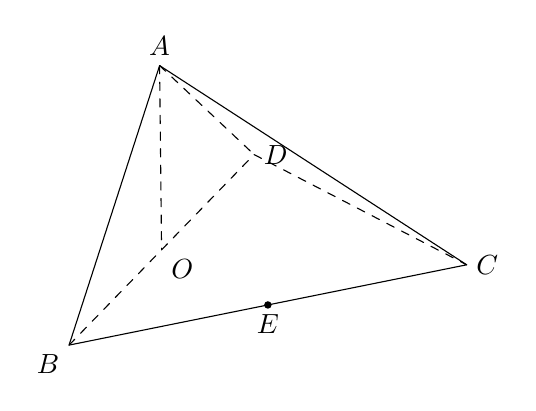
\begin{tikzpicture}[line cap=round,line join=round]
  % Schematic positions only; no lengths or angles are encoded.
  \coordinate (A) at (1.15,3.55);
  \coordinate (B) at (0,0);
  \coordinate (C) at (5.05,1.02);
  \coordinate (D) at (2.35,2.42);
  \coordinate (O) at (1.175,1.21);
  \coordinate (E) at (2.525,0.51);

  % Visible edges
  \draw (A) -- (B) -- (C) -- cycle;

  % Hidden edges and the indicated segment AO
  \draw[dashed] (A) -- (D);
  \draw[dashed] (B) -- (D);
  \draw[dashed] (D) -- (C);
  \draw[dashed] (A) -- (O);

  \fill (E) circle (1.35pt);
  \node[above]       at (A) {$A$};
  \node[below left]  at (B) {$B$};
  \node[right]       at (C) {$C$};
  \node[right]       at (D) {$D$};
  \node[below right] at (O) {$O$};
  \node[below]       at (E) {$E$};
\end{tikzpicture}
\end{center}
\nopagebreak[4]
\Needspace{4\baselineskip}
\textbf{解析}

\Needspace{5\baselineskip}
\textbf{(1)} 以 $O$ 为原点，令 $BD$ 为 $x$ 轴并取
\nopagebreak[4]
\[
B=(-1,0,0),\quad D=(1,0,0),\quad C=(0,\sqrt3,0),\quad A=(0,0,1).
\]
这些坐标满足题设各边长：$BD=BC=CD=2$，$AB=AD=\sqrt2$，$CA=2$；因此 $BCD$ 在 $z=0$ 平面内且 $AO$ 为 $z$ 轴，得到 $AO\perp$ 平面 $BCD$。

\textbf{(2)} 可取 $AB$、$CD$ 的方向向量分别为 $(-1,0,-1)$、$(1,-\sqrt3,0)$，点积为 $-1$，模长分别为 $\sqrt2$ 和 $2$。两异面直线所成角取锐角，故其余弦为 $1/(2\sqrt2)$，角为 $\arccos\frac1{2\sqrt2}$。

\Needspace{5\baselineskip}
\textbf{(3)} $E$ 是 $BC$ 中点，坐标为 $(-1/2,\sqrt3/2,0)$。过 $A,C,D$ 的平面方程为 $x+y/\sqrt3+z=1$。代入点到平面距离公式，距离为
\nopagebreak[4]
\[
\frac{| -1/2+1/2-1|}{\sqrt{1+1/3+1}}=\sqrt{\frac37}.
\]
\nopagebreak[4]
\begin{center}% Schematic reconstruction of the visible Q19 diagram (2006 Fujian arts paper).
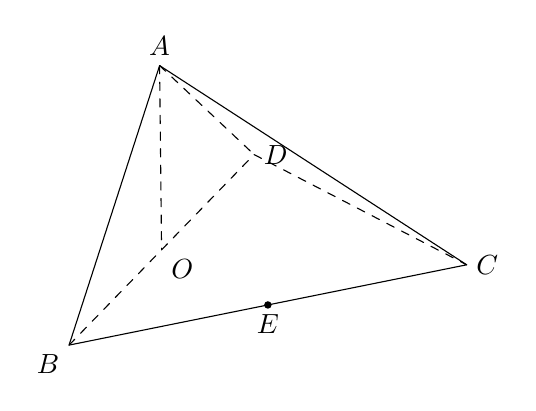
\begin{tikzpicture}[line cap=round,line join=round]
  % Schematic positions only; no lengths or angles are encoded.
  \coordinate (A) at (1.15,3.55);
  \coordinate (B) at (0,0);
  \coordinate (C) at (5.05,1.02);
  \coordinate (D) at (2.35,2.42);
  \coordinate (O) at (1.175,1.21);
  \coordinate (E) at (2.525,0.51);

  % Visible edges
  \draw (A) -- (B) -- (C) -- cycle;

  % Hidden edges and the indicated segment AO
  \draw[dashed] (A) -- (D);
  \draw[dashed] (B) -- (D);
  \draw[dashed] (D) -- (C);
  \draw[dashed] (A) -- (O);

  \fill (E) circle (1.35pt);
  \node[above]       at (A) {$A$};
  \node[below left]  at (B) {$B$};
  \node[right]       at (C) {$C$};
  \node[right]       at (D) {$D$};
  \node[below right] at (O) {$O$};
  \node[below]       at (E) {$E$};
\end{tikzpicture}
\end{center}
\nopagebreak[4]
\gkanswer{答案（1）：证明见解析。}

\gkanswer{答案（2）：$\arccos\dfrac1{2\sqrt2}$}

\gkanswer{答案（3）：$\sqrt{\dfrac37}$}

\end{answer}
\begin{answer}
\gksolhead{20}{}

\textbf{题目}：

\Needspace{5\baselineskip}
已知椭圆
\nopagebreak[4]
\[
\frac{x^2}{2}+y^2=1
\]
的左焦点为 $F$，$O$ 为坐标原点。

（1） 求过点 $O$、$F$，并且与椭圆的左准线 $l$ 相切的圆的方程；

（2） 设过点 $F$ 且不与坐标轴垂直的直线交椭圆于 $A$、$B$ 两点，并且线段 $AB$ 的中点在直线 $x+y=0$ 上，求直线 $AB$ 的方程。
\nopagebreak[4]
\begin{center}% Source schematic: 2006 Fujian arts paper, Q20, source PDF page 2.
% Include inside a document that loads TikZ.
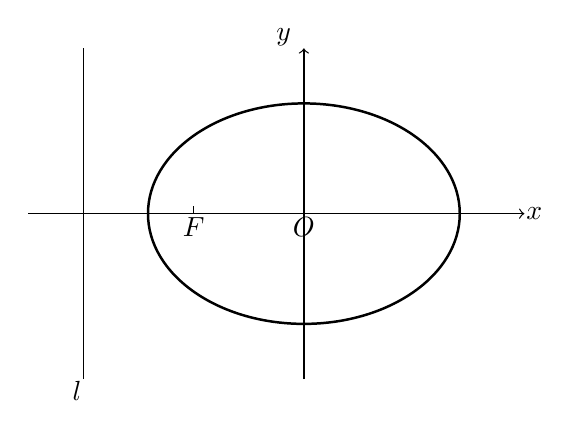
\begin{tikzpicture}[x=1.4cm,y=1.4cm,line cap=butt,line join=round]
  % Coordinate axes: arrows point in the positive directions only.
  \draw[->,line width=0.45pt] (-2.5,0) -- (2,0);
  \draw[->,line width=0.45pt] (0,-1.5) -- (0,1.5);

  % Left directrix, shown as a plain solid vertical line.
  \draw[line width=0.45pt] (-2,-1.5) -- (-2,1.5);

  % Ellipse x^2/2 + y^2 = 1, with the left focus tick on the x-axis.
  \draw[line width=0.9pt] (0,0) ellipse [x radius=1.4142,y radius=1];
  \draw[line width=0.45pt] (-1,0) -- (-1,0.07);

  % Labels copied from the schematic.
  \node[above left,inner sep=0.5pt] at (-0.1,1.5) {$y$};
  \node[right,inner sep=0.5pt] at (2,0) {$x$};
  \node[below,inner sep=0.5pt] at (-1,-0.02) {$F$};
  \node[below,inner sep=0.5pt] at (0,-0.02) {$O$};
  \node[below left,inner sep=0.5pt] at (-2,-1.5) {$l$};
\end{tikzpicture}
\end{center}
\nopagebreak[4]
\Needspace{4\baselineskip}
\textbf{解析}

椭圆 $x^2/2+y^2=1$ 的焦距参数 $c=1$，故 $F=(-1,0)$，左准线为 $x=-2$。
\nopagebreak[4]
\begin{center}% Source schematic: 2006 Fujian arts paper, Q20, source PDF page 2.
% Include inside a document that loads TikZ.
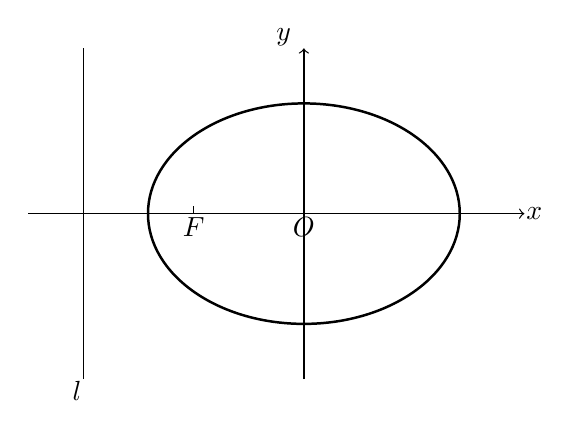
\begin{tikzpicture}[x=1.4cm,y=1.4cm,line cap=butt,line join=round]
  % Coordinate axes: arrows point in the positive directions only.
  \draw[->,line width=0.45pt] (-2.5,0) -- (2,0);
  \draw[->,line width=0.45pt] (0,-1.5) -- (0,1.5);

  % Left directrix, shown as a plain solid vertical line.
  \draw[line width=0.45pt] (-2,-1.5) -- (-2,1.5);

  % Ellipse x^2/2 + y^2 = 1, with the left focus tick on the x-axis.
  \draw[line width=0.9pt] (0,0) ellipse [x radius=1.4142,y radius=1];
  \draw[line width=0.45pt] (-1,0) -- (-1,0.07);

  % Labels copied from the schematic.
  \node[above left,inner sep=0.5pt] at (-0.1,1.5) {$y$};
  \node[right,inner sep=0.5pt] at (2,0) {$x$};
  \node[below,inner sep=0.5pt] at (-1,-0.02) {$F$};
  \node[below,inner sep=0.5pt] at (0,-0.02) {$O$};
  \node[below left,inner sep=0.5pt] at (-2,-1.5) {$l$};
\end{tikzpicture}
\end{center}
\nopagebreak[4]
\Needspace{5\baselineskip}
\textbf{(1)} 过 $O,F$ 的圆心在 $x=-1/2$ 上。设圆心为 $(-1/2,t)$，半径平方为 $1/4+t^2$。与 $x=-2$ 相切要求半径为 $3/2$，于是 $1/4+t^2=9/4$，即 $t=\pm\sqrt2$。所求两圆为
\nopagebreak[4]
\[
\left(x+\frac12\right)^2+(y-\sqrt2)^2=\frac94,\qquad
\left(x+\frac12\right)^2+(y+\sqrt2)^2=\frac94.
\]

\Needspace{5\baselineskip}
\textbf{(2)} 设直线斜率为 $k$。因直线不与坐标轴垂直，$k$ 有限且 $k\ne0$，可写为 $y=k(x+1)$。代入椭圆得
\nopagebreak[4]
\[
\left(\frac12+k^2\right)x^2+2k^2x+(k^2-1)=0.
\]
两交点横坐标的平均值为 $\bar x=-2k^2/(1+2k^2)$，而 $\bar y=k(\bar x+1)=k/(1+2k^2)$。条件 $\bar x+\bar y=0$ 给出 $k(1-2k)=0$。因 $k\ne0$，$k=1/2$，故直线为 $y=(x+1)/2$，即 $x-2y+1=0$。代入所得二次方程判别式为正，确有两个不同交点。

\gkanswer{答案（1）：$\left(x+\dfrac12\right)^2+(y-\sqrt2)^2=\dfrac94$ 或 $\left(x+\dfrac12\right)^2+(y+\sqrt2)^2=\dfrac94$。}

\gkanswer{答案（2）：$x-2y+1=0$}

\end{answer}
\begin{answer}
\gksolhead{21}{}

\textbf{题目}：

已知 $f(x)$ 是二次函数，不等式 $f(x)<0$ 的解集是 $(0,5)$，且 $f(x)$ 在区间 $[-1,4]$ 上的最大值是 12。

（1） 求 $f(x)$ 的解析式；

\Needspace{5\baselineskip}
（2） 是否存在自然数 $m$，使得方程
\nopagebreak[4]
\[
f(x)+\frac{37}{x}=0
\]
在区间 $(m,m+1)$ 内有且只有两个不等的实数根？若存在，求出所有 $m$ 的值；若不存在，说明理由。

\Needspace{4\baselineskip}
\textbf{解析}

\textbf{(1)} 由 $f(x)<0$ 的解集为 $(0,5)$，设 $f(x)=a x(x-5)$，$a>0$。开口向上的二次函数在 $[-1,4]$ 上最大值取于端点；$f(-1)=6a$、$f(4)=-4a$，故 $6a=12$，得 $f(x)=2x^2-10x$。

\textbf{(2)} 在自然数区间中 $x>0$，原方程等价于 $g(x)=2x^3-10x^2+37=0$。导数 $g'(x)=2x(3x-10)$，故 $g$ 在 $(0,10/3)$ 递减、在 $(10/3,+\infty)$ 递增。又 $g(3)=1>0$、$g(10/3)=-1/27<0$、$g(4)=5>0$，所以恰有两个正根，且均在 $(3,4)$，在该开区间内有且仅有两个根。其余正整数单位区间不可能含两个根，故 $m=3$。

\gkanswer{答案（1）：$f(x)=2x^2-10x$}

\gkanswer{答案（2）：$m=3$}

\end{answer}
\begin{answer}
\gksolhead{22}{}

\textbf{题目}：

已知数列 $\{a_n\}$ 满足 $a_1=1$，$a_2=3$，$a_{n+2}=3a_{n+1}-2a_n\ (n\in\mathbb{N}^*)$。

（1） 证明：数列 $\{a_{n+1}-a_n\}$ 是等比数列；

（2） 求数列 $\{a_n\}$ 的通项公式；

\Needspace{5\baselineskip}
（3） 若数列 $\{b_n\}$ 满足
\nopagebreak[4]
\[
4^{b_1-1}4^{b_2-1}\cdots 4^{b_n-1}=(a_n+1)^{b_n}\quad(n\in\mathbb{N}^*),
\]
证明：$\{b_n\}$ 是等差数列。

\Needspace{4\baselineskip}
\textbf{解析}

\textbf{(1)} 令 $d_n=a_{n+1}-a_n$。递推式给出 $d_{n+1}=2a_{n+1}-2a_n=2d_n$，且 $d_1=2$，所以该数列为首项、公比均为 $2$ 的等比数列。

\textbf{(2)} $a_n=1+\sum_{j=1}^{n-1}2^j=2^n-1$。

\Needspace{5\baselineskip}
\textbf{(3)} 令 $S_n=\sum_{j=1}^n b_j$。由 $a_n+1=2^n$，题设等式化为 $4^{S_n-n}=4^{nb_n/2}$，即
\nopagebreak[4]
\[
S_n=n+\frac n2 b_n.
\]
取 $n=1$ 得 $b_1=2$。对 $n\ge3$，将上式分别用于 $n$ 与 $n-1$ 并相减，得 $(n-2)b_n=(n-1)b_{n-1}-2$。令 $c_n=b_n-2$，则 $(n-2)c_n=(n-1)c_{n-1}$，故 $c_n/(n-1)$ 对 $n\ge2$ 为常数。于是 $b_n=2+(n-1)(b_2-2)$，所以 $\{b_n\}$ 为等差数列。注意 $n=2$ 时原关系仅为恒等式，不会额外限定其公差。

\gkanswer{答案（1）：数列 $\{a_{n+1}-a_n\}$ 首项为 $2$、公比为 $2$。}

\gkanswer{答案（2）：$a_n=2^n-1$}

\gkanswer{答案（3）：$\{b_n\}$ 为等差数列，可写为 $b_n=2+(n-1)(b_2-2)$。}

\end{answer}